The general objective of this thesis is to provide tools that will expose cache
coherence interference to an applicant seeking the certification of system with
multi-core processor, thereby contributing to the resolution of the
\textit{Resource Usage 3} requirement. Indeed, that requirement asks that the
applicant identifies all interference and its impact on the applications.

As the necessary notions have now been introduced, the problem statement from
Section~\ref{sec:intro:prob_statement} and the proposed solution can be
presented in more details. Thus, this chapter clarifies the scope of this
thesis and provides an explanation of how its contributions form a framework
that exposes cache coherence interference.

\stopallthesefloats
\section{Tasks Required of the Applicant}
To fulfill the \textit{RU3} objective, the applicant has to catalog all
interference channels, as well as all interference, and to mitigate them so that
they do not prevent the applications from otherwise fulfilling other
requirements. To determine where the interference is and how much of an impact
they could potentially have, an understanding of the architecture's mechanisms
is required. When the mechanisms that generate them are not removed all
together, the applicant must be able to quantify their impact on the running
software.

\subsection{Coherence Protocol Identification}
\label{aaa:identification}
Ideally, the solution would simply be to consult the architecture's
documentation, where the mechanisms would be described in details and,
hopefully, so would all interference inducing behaviors. However, actual
documentation for COTS processors do not generally include details on cache
coherence. This is the first issue addressed in this thesis: how can one be sure
of their understanding of the architecture's cache coherence mechanisms?
On this topic, the contribution this thesis makes is to point out a missing
preliminary step, and propose a strategy for it. Indeed, instead of focusing on
the already resolved issue of measuring the time required to perform an access,
or the bandwidth such accesses would have, the issue of incorrect assumptions on
the architecture's cache coherence mechanisms is addressed. In effect, because
the documentation of the implemented cache coherence mechanisms is not precise,
there is a strong risk of mismatch between what the architecture actually
performs and what is being tested, for why would one test the performance of
something they understand not to be present?

For example, if a \textit{MESI} architecture was benchmarked as if it were a
\textit{MSI} one, the interference generated by having two caches each perform
an initial read on a memory would, for one of the two caches, not be the same as
with a true \textit{MSI} architecture. Not realizing this would lead the
applicant to wrongly characterize the architecture. They could incorrectly
underestimate the cost of simultaneous reading, if the measures happened to be
done on the second cache to complete reading, as the data would then be provided
by the first cache. Since this is happens only in special cases with the
\textit{MESI} protocol, to consider this measure representative of the general
case of parallel reading would lead to a completely incorrect analysis of the
effects of interference. Since these special cases are not found within the
\textit{MSI} cache protocol, the applicant would not know to be wary of them.

Ensuring that the architecture's cache coherence mechanisms have properly been
identified and their characteristics measured is a necessary step for the
analysis of the architecture. It is however not sufficient to infer what
interference the architecture's mechanisms will generate, nor how it will
affect the execution of the applications.

\subsection{Measuring the Impact of Interference of the Software}
\begin{definition}[Impact of Interference]
\label{sec:impact_of_interference}
The impact of an interference is a quantification of the temporal effects of
interference on an application's execution. More precisely, it is the amount of
additional CPU cycles required to execute a given fragment of the application
compared its execution in isolation.
\end{definition}

\begin{figure}[hbt!]
\begin{center}
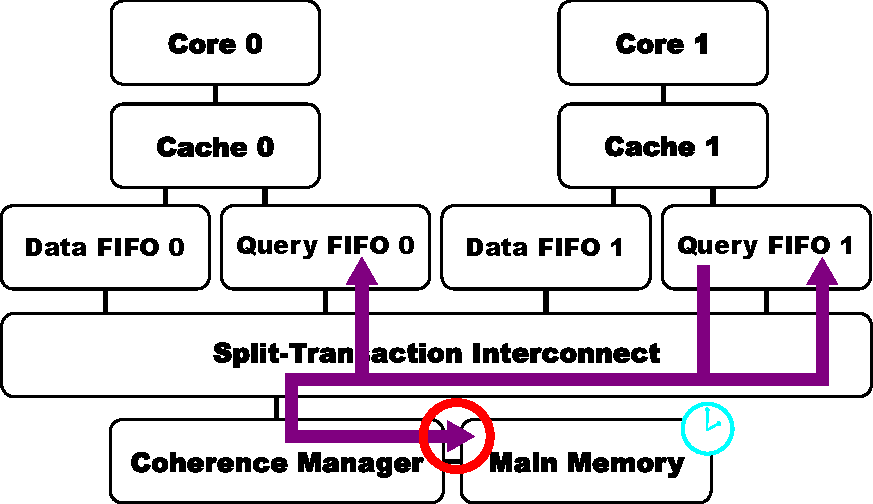
\includegraphics[width=0.6\textwidth]{\chapterdirectory/figure/demo_arch1.pdf}
\end{center}
\caption{Second Example of Interference}
\label{fig:second_intro:interference_example2}
\end{figure}

\begin{example}[Impact of Interference]
The interference from Example~\ref{ex:second_intro:interference}, by itself, may
not be noticeable by \textit{Core 1} if it lasts less than a cycle. However, an
impact could be measured in a follow-up interference: once \textit{Cache 0}'s
query reaches the main memory, it stays busy for an appreciable amount of time
before becoming available once again (see
Figure~\ref{fig:second_intro:interference_example2}). Here also, \textit{Cache
1}'s query ends up delayed. In effect, if the main memory stays busy for 12 CPU
cycles before \textit{Cache 1}'s query is considered, then the impact of that
interference is the 12 CPU cycles delay.
\end{example}

Even when the architecture's mechanisms have been fully identified, predicting
the impact of interference on the execution of programs is not an issue
currently resolved by the existing literature. Restricting this issue to caches
in which coherence has been disabled still does not lead to a perfect solution.
Indeed, this was already problematic in single core systems in which multiple
applications share a same cache. The issue being that some aspects of the
architecture will still remain slightly ambiguous, and so the exact order in
which events occur cannot be determined.  Depending on the placement and
replacement policies of the cache, this makes it difficult to know the content
of the cache at any given time.  Cache coherence adds to the number of events
that can occur, and make the content of other caches decide whether events
occur, thus tremendously complexifying the issue. Ignoring the effects of
such mechanisms would quickly lead to either incorrect or unusable execution
time estimations, as any memory access would have a seemingly random temporal
cost as the then invisible coherence states would influence it. The existing
literature offers compromises: either analyzing strategies that will yield
overly pessimistic WCET, or restrictions to eliminate sources of interference so
that their effects need not be taken into account.  The available analysis
strategies do not address cache coherence. Some of the approaches using
restrictions do take cache coherence into account, but only through hardware
modifications, which is not deemed acceptable in an aeronautical context. This
thesis proposes an approach to analyze the effects of cache coherence. The idea
is to have an accurate representation of all mechanisms that are known and use
formal methods to ensure all possible behaviors of the mechanisms for which
ambiguities remain are explored.

\stopallthesefloats
\section{Proposed Solution}
In effect, this thesis proposes to tackle the issue of interference generated by
cache coherence by first ensuring complete understanding of the architecture's
cache coherence mechanisms through the proposed identification strategy, then
using existing approaches to measure the timing characteristics of these
mechanisms, to finally use formal methods on a model based on what is presented
in this thesis in order to infer the effects of the interference on the running
software.
